\PassOptionsToPackage{svgnames,dvipsnames,svgnames}{xcolor}

% From https://pldi19.sigplan.org/track/pldi-2019-papers#Call-for-Papers
\documentclass[sigplan,10pt,nonacm]{acmart}
\settopmatter{printfolios=true,printccs=false,printacmref=false}

%\documentclass[acmsmall,review,anonymous]{acmart}

%% For double-blind review submission, w/o CCS and ACM Reference (max submission space)
%% \documentclass[sigplan,review,anonymous]{acmart}\settopmatter{printfolios=true,printccs=false,printacmref=false}
%% For double-blind review submission, w/ CCS and ACM Reference
%\documentclass[sigplan,review,anonymous]{acmart}\settopmatter{printfolios=true}
%% For single-blind review submission, w/o CCS and ACM Reference (max submission space)
%\documentclass[sigplan,review]{acmart}\settopmatter{printfolios=true,printccs=false,printacmref=false}
%% For single-blind review submission, w/ CCS and ACM Reference
%\documentclass[sigplan,review]{acmart}\settopmatter{printfolios=true}
%% For final camera-ready submission, w/ required CCS and ACM Reference
%\documentclass[sigplan]{acmart}\settopmatter{}


%% Conference information
%% Supplied to authors by publisher for camera-ready submission;
%% use defaults for review submission.
\acmConference[PL'18]{ACM SIGPLAN Conference on Programming Languages}{January 01--03, 2018}{New York, NY, USA}
\acmYear{2018}
\acmISBN{} % \acmISBN{978-x-xxxx-xxxx-x/YY/MM}
\acmDOI{} % \acmDOI{10.1145/nnnnnnn.nnnnnnn}
\startPage{1}

%% Copyright information
%% Supplied to authors (based on authors' rights management selection;
%% see authors.acm.org) by publisher for camera-ready submission;
%% use 'none' for review submission.
\setcopyright{none}
%\setcopyright{acmcopyright}
%\setcopyright{acmlicensed}
%\setcopyright{rightsretained}
%\copyrightyear{2018}           %% If different from \acmYear

%% Bibliography style
\bibliographystyle{ACM-Reference-Format}
%% Citation style
%\citestyle{acmauthoryear}  %% For author/year citations
%\citestyle{acmnumeric}     %% For numeric citations
%\setcitestyle{nosort}      %% With 'acmnumeric', to disable automatic
                            %% sorting of references within a single citation;
                            %% e.g., \cite{Smith99,Carpenter05,Baker12}
                            %% rendered as [14,5,2] rather than [2,5,14].
%\setcitesyle{nocompress}   %% With 'acmnumeric', to disable automatic
                            %% compression of sequential references within a
                            %% single citation;
                            %% e.g., \cite{Baker12,Baker14,Baker16}
                            %% rendered as [2,3,4] rather than [2-4].


%% Some recommended packages.
\usepackage{booktabs}   %% For formal tables:
                        %% http://ctan.org/pkg/booktabs
\usepackage{subcaption} %% For complex figures with subfigures/subcaptions
                        %% http://ctan.org/pkg/subcaption

%% Cyrus packages
\usepackage{microtype}
\usepackage{mdframed}
\usepackage{colortab}
\usepackage{mathpartir}
\usepackage{enumitem}
\usepackage{bbm}
\usepackage{stmaryrd}
\usepackage{mathtools}
\usepackage{leftidx}
\usepackage{todonotes}
\usepackage{xspace}
\usepackage{wrapfig}


\usepackage{listings}%
\lstloadlanguages{ML}
\lstset{tabsize=2, 
basicstyle=\footnotesize\ttfamily, 
% keywordstyle=\sffamily,
commentstyle=\itshape\ttfamily\color{gray}, 
stringstyle=\ttfamily\color{purple},
mathescape=false,escapechar=\#,
numbers=left, numberstyle=\scriptsize\color{gray}\ttfamily, language=ML, showspaces=false,showstringspaces=false,xleftmargin=10pt, 
morekeywords={string, float, int},
classoffset=0,belowskip=\smallskipamount, aboveskip=\smallskipamount,
moredelim=**[is][\color{red}]{SSTR}{ESTR}
}
\newcommand{\li}[1]{\lstinline[basicstyle=\ttfamily\fontsize{9pt}{1em}\selectfont]{#1}}
\newcommand{\lismall}[1]{\lstinline[basicstyle=\ttfamily\fontsize{9pt}{1em}\selectfont]{#1}}

%% Joshua Dunfield macros
\def\OPTIONConf{1}%
\usepackage{joshuadunfield}

%% Can remove this eventually
\usepackage{blindtext}

\usepackage{enumitem}

%%%%%%%%%%%%%%%%%%%%%%%%%%%%%%%%%%%%%%%%%%%%%%%%%%%%%%%%%%%%%%%%%%%%%%%%%%%%%
%% Matt says: Cyrus, this package `adjustbox` seems directly related
%% to the `clipbox` error; To get rid of the error, I moved it last
%% (after other usepackages) and I added the line just above it, which
%% permits it to redefine `clipbox` (apparently also defined in
%% `pstricks`, and due to latex's complete lack of namespace
%% management, these would otherwise names clash).
\let\clipbox\relax
\usepackage[export]{adjustbox}% http://ctan.org/pkg/adjustbox
%%%%%%%%%%%%%%%%%%%%%%%%%%%%%%%%%%%%%%%%%%%%%%%%%%%%%%%%%%%%%%%%%%%%%%%%%%%%%%%%%


%%%%%%%%%%%%%%%%%%%%%%%%%%%%%%%%%%%%%%%%%%%%%%%%%%%%%%%%%%%%%%%%%%%%%%%%%%%%%%%%%
%\usepackage{draftwatermark}
%\SetWatermarkText{DRAFT}
%\SetWatermarkScale{1}
%%%%%%%%%%%%%%%%%%%%%%%%%%%%%%%%%%%%%%%%%%%%%%%%%%%%%%%%%%%%%%%%%%%%%%%%%%%%%%%%%


% A macro for the name of the system being described by ``this paper''
\newcommand{\HazelnutLive}{\textsf{Hazelnut Live}\xspace}
\newcommand{\Hazelnut}{\textsf{Hazelnut}\xspace}
% The mockup, work-in-progress system.
\newcommand{\Hazel}{\textsf{Hazel}\xspace}

% \newtheorem{theorem}{Theorem}[chapter]
% \newtheorem{lemma}[theorem]{Lemma}
% \newtheorem{corollary}[theorem]{Corollary}
% \newtheorem{definition}[theorem]{Definition}
% \newtheorem{assumption}[theorem]{Assumption}
% \newtheorem{condition}[theorem]{Condition}

\newtheoremstyle{slplain}% name
  {.15\baselineskip\@plus.1\baselineskip\@minus.1\baselineskip}% Space above
  {.15\baselineskip\@plus.1\baselineskip\@minus.1\baselineskip}% Space below
  {\slshape}% Body font
  {\parindent}%Indent amount (empty = no indent, \parindent = para indent)
  {\bfseries}%  Thm head font
  {.}%       Punctuation after thm head
  { }%      Space after thm head: " " = normal interword space;
        %       \newline = linebreak
  {}%       Thm head spec
\theoremstyle{slplain}
\newtheorem{thm}{Theorem}  % Numbered with the equation counter
\numberwithin{thm}{section}
\newtheorem{defn}[thm]{Definition}
\newtheorem{lem}[thm]{Lemma}
\newtheorem{prop}[thm]{Proposition}
% \newtheorem{cor}[section]{Corollary}     
% \newtheorem{lem}[section]{Lemma}         
% \newtheorem{prop}[section]{Proposition}  

% \setlength{\abovedisplayskip}{0pt}
% \setlength{\belowdisplayskip}{0pt}
% \setlength{\abovedisplayshortskip}{0pt}
% \setlength{\belowdisplayshortskip}{0pt}



\makeatletter\if@ACM@journal\makeatother
%% Journal information (used by PACMPL format)
%% Supplied to authors by publisher for camera-ready submission
\acmJournal{PACMPL}
\acmVolume{1}
\acmNumber{1}
\acmArticle{1}
\acmYear{2018}
\acmMonth{3}
\acmDOI{10.1145/nnnnnnn.nnnnnnn}
\startPage{1}
\else\makeatother
%% Conference information (used by SIGPLAN proceedings format)
%% Supplied to authors by publisher for camera-ready submission
% \acmConference[]{ACM SIGPLAN Conference on Programming Languages}{January 01--03, 2017}{New York, NY, USA}

\acmYear{2018}
\acmISBN{978-x-xxxx-xxxx-x/YY/MM}
\acmDOI{10.1145/nnnnnnn.nnnnnnn}
\startPage{1}
\fi


%% Copyright information
%% Supplied to authors (based on authors' rights management selection;
%% see authors.acm.org) by publisher for camera-ready submission
\setcopyright{none}             %% For review submission
%\setcopyright{acmcopyright}
%\setcopyright{acmlicensed}
%\setcopyright{rightsretained}
%\copyrightyear{2017}           %% If different from \acmYear


\fancyfoot{} % suppresses the footer (also need \thispagestyle{empty} after \maketitle below)


%% Bibliography style
\bibliographystyle{ACM-Reference-Format}
%% Citation style
%% Note: author/year citations are required for papers published as an
%% issue of PACMPL.
\citestyle{acmauthoryear}   %% For author/year citations

% !TEX root = main.tex

\newcommand{\mynote}[3]{\textcolor{#3}{\textsf{{#2}}}}
\newcommand{\rkc}[1]{\mynote{rkc}{#1}{blue}}
\newcommand{\cy}[1]{\mynote{cy}{#1}{purple}}
\newcommand{\mah}[1]{\mynote{cy}{#1}{green}}
\newcommand{\matt}[1]{{\color{blue}{\textit{Matt:~#1}}}}

\newcommand{\cvert}{{\,{\vert}\,}}

%% https://tex.stackexchange.com/questions/9796/how-to-add-todo-notes
\newcommand{\rkcTodo}[1]{\todo[linecolor=blue,backgroundcolor=blue!25,bordercolor=blue]{#1}}

\newcommand{\mattTodo}[1]{\todo[linecolor=green,backgroundcolor=green!2,bordercolor=green]{\tiny\textit{#1}}}
\newcommand{\mattOmit}[1]{\colorbox{yellow}{(Matt omitted stuff here)}}

\def\parahead#1{\paragraph{\textbf{#1.}}}
%% \def\paraheadNoDot#1{\paragraph{{\textbf{#1}}}}
\def\subparahead#1{\paragraph{\textit{#1.}}}
%% \def\paraheadindent#1{\paragraph{}\textit{#1.}}
%% \def\paraheadindentnodot#1{\paragraph{}\textit{#1}}

% \newcommand{\ie}{{\emph{i.e.}}}
% \newcommand{\eg}{{\emph{e.g.}}}
% \newcommand{\etc}{{\emph{etc.}}}
% \newcommand{\cf}{{\emph{cf.}}}
% \newcommand{\etal}{{\emph{et al.}}}

%% \newcommand{\hazel}{\ensuremath{\textsc{Hazel}}}
%% \newcommand{\sns}{\ensuremath{\textsc{Sketch-n-Sketch}}}
%% \newcommand{\deuce}{\ensuremath{\textsc{Deuce}}}
\newcommand{\Elm}{\ensuremath{\textsf{Elm}}}
\newcommand{\sns}{\ensuremath{\textrm{Sketch-n-Sketch}}}
\newcommand{\deuce}{\ensuremath{\textrm{Deuce}}}

\newcommand{\sectionDescription}[1]{\section{#1}}
\newcommand{\subsectionDescription}[1]{\subsection{#1}}
\newcommand{\subsubsectionDescription}[1]{\subsubsection{#1}}
%% \newcommand{\subsectionDescription}[1]{\subsection*{#1}}
\newcommand{\suppMaterials}{the Supplementary Materials}

\newcommand{\defeq}{\overset{\textrm{def}}{=}}

\newcommand{\eap}{action suggestion panel\xspace}
\newcommand{\Eap}{Action suggestion panel\xspace}

\newcommand{\myfootnote}[1]{\footnote{ #1}}

\def\sectionautorefname{Section}
\def\subsectionautorefname{Section}
\def\subsubsectionautorefname{Section}

\newcommand{\code}[1]{\lstinline{#1}}

% Make italic?
%\newcommand{\Property}[1]{\emph{#1}}
\newcommand{\Property}[1]{\textrm{#1}}

% Calling out Cyrus's favorite verb, 'to be' ;)
\newcommand{\IS}{\colorbox{red}{is}\xspace}

\newcommand{\codeSize}
  %% {\footnotesize}
  {\small}

%\newcommand{\JoinTypes}[2]{\textsf{join}~~#1~~#2}
\newcommand{\JoinTypes}[2]{\textsf{join}(#1,#2)}

%%%%%%%%%%%%%%%%%%%%%%%%%%%%%%%%%%%%%%%%%%%%%%%%%%%%%%%%%%%%%%%%%%%%%%%%%%%%%%%%
%% Spacing

\newcommand{\sep}{\hspace{0.06in}}
\newcommand{\sepPremise}{\hspace{0.20in}}
\newcommand{\hsepRule}{\hspace{0.20in}}
\newcommand{\vsepRuleHeight}{0.08in}
\newcommand{\vsepRule}{\vspace{\vsepRuleHeight}}
\newcommand{\miniSepOne}{\hspace{0.01in}}
\newcommand{\miniSepTwo}{\hspace{0.02in}}
\newcommand{\miniSepThree}{\hspace{0.03in}}
\newcommand{\miniSepFour}{\hspace{0.04in}}
\newcommand{\miniSepFive}{\hspace{0.05in}}

%%%%%%%%%%%%%%%%%%%%%%%%%%%%%%%%%%%%%%%%%%%%%%%%%%%%%%%%%%%%%%%%%%%%%%%%%%%%%%%%

% \lstset{
% %mathescape=true,basicstyle=\fontsize{8}{9}\ttfamily,
% literate={=>}{$\Rightarrow$}2
%          {<=}{$\leq$}2
%          {->}{${\rightarrow}$}1
%          {\\\\=}{\color{red}{$\lambda$}}2
%          {\\\\}{$\lambda$}2
%          {**}{$\times$}2
%          {*.}{${\color{blue}{\texttt{*.}}}$}2
%          {+.}{${\color{blue}{\texttt{+.}}}$}2
%          {<}{${\color{green}{\lhd}}$}1
%          {>?}{${\color{green}{\rhd}}$?}2
%          {<<}{${\color{green}{\blacktriangleleft}}$}1
%          {>>?}{${\color{green}{\blacktriangleright}}$?}2
%          {\{}{${\color{blue}{\{}}$}1
%          {\}}{${\color{blue}{\}}}$}1
%          {[}{${\color{purple}{[}}$}1
%          {]}{${\color{purple}{]}}$}1
%          {(}{${\color{darkgray}{\texttt{(}}}$}1
%          {)}{${\color{darkgray}{\texttt{)}}}$}1
%          {]]}{${\color{gray}{\big(}}$}1
%          {]]}{${\color{gray}{\big)}}$}1
% }

% !TEX root = hazelnut-dynamics.tex

% \newcommand{\Label}[1]{\vspace{-20px}\label{#1}%
%   {\small\textcolor{cyan}{(\texttt{#1})}}\vspace{20px}%
% }

\newcommand{\cmttclo}[2]{\mathsf{clo}(#1, #2)}

% \newcommand{\CaptionLabel}[2]{
%   \caption{#1 {\small\textcolor{cyan}{(#2)}}}
%   \label{#2}}
\newcommand{\CaptionLabel}[2]{
  \caption{#1}
  \label{#2}}

% Violet hotdogs; highlight color helps distinguish them
\newcommand{\llparenthesiscolor}{\textcolor{violet}{\llparenthesis}}
\newcommand{\rrparenthesiscolor}{\textcolor{violet}{\rrparenthesis}}
% \newcommand{\llparenthesiscolor}{\textcolor{red}{\lfloor}}
% \newcommand{\rrparenthesiscolor}{\textcolor{red}{\rfloor}}

%% TODO if feeling really obsessive, use the following in place of x,u,c,b
\newcommand{\varVar}{x}
\newcommand{\varHole}{u}
\newcommand{\econst}{c}
\newcommand{\tbase}{b}

% HTyp and HExp
\newcommand{\isComplete}[1]{#1~\mathsf{complete}}

% HTyp
\newcommand{\htau}{\tau}
\newcommand{\tarr}[2]{#1 \rightarrow #2}
%\newcommand{\tsum}[2]{#1 + #2}
\newcommand{\tprod}[2]{#1 \times #2}
\newcommand{\tnum}{\texttt{num}}
\newcommand{\tb}{\texttt{b}}
\newcommand{\tehole}{\llparenthesiscolor\rrparenthesiscolor}
\newcommand{\tsum}[2]{{#1} + {#2}}

\newcommand{\tconsistent}[2]{#1 \sim #2}
\newcommand{\tinconsistent}[2]{#1 \nsim #2}

% HExp
\newcommand{\hexp}{e}
\newcommand{\hlam}[2]{\lambda #1.#2}
\newcommand{\halam}[3]{\lambda #1{:}#2.#3}
\newcommand{\hap}[2]{#1(#2)}
\newcommand{\hapP}[2]{(#1)~(#2)} % Extra paren around function term
\newcommand{\hpair}[2]{(#1, #2)}
\newcommand{\hprj}[2]{\mathsf{prj}_{#1}(#2)}
\newcommand{\lblL}{\mathsf{L}}
\newcommand{\lblR}{\mathsf{R}}
\newcommand{\hnum}[1]{\underline{#1}}
%\newcommand{\hcase}[5]{\mathsf{case}\,#1\,\mathsf{of}\,#2\Rightarrow#3~\vert~#4\Rightarrow#5}
\newcommand{\hadd}[2]{#1 + #2}
\newcommand{\hehole}[1]{\llparenthesiscolor\rrparenthesiscolor^{#1}}
% \newcommand{\hhole}[1]{\setlength{\fboxsep}{0pt}\fcolorbox{red}{white}{\vphantom{)}$#1$}}
\newcommand{\hhole}[2]{\llparenthesiscolor#1\rrparenthesiscolor^{#2}}
% \newcommand{\hhole}[1]{
  % \setlength{\fboxsep}{0pt}
  % \colorbox{violet!10!white!100}{\ensuremath{\llparenthesiscolor#1\rrparenthesiscolor}}}
\newcommand{\hindet}[1]{\lceil#1\rceil}
%\newcommand{\hinj}[2]{\texttt{inj}_{#1}({#2})}
\newcommand{\hinL}[1]{\mathsf{inl}(#1)}
\newcommand{\hinR}[1]{\mathsf{inr}(#1)}
\newcommand{\hcase}[5]{\texttt{case}({#1},{#2}.{#3},{#4}.{#5})}

\newcommand{\hGamma}{\Gamma}
\newcommand{\EmptyhGamma}{\emptyset} % From hand-written notes, Canonical forms lemma; page 14
\newcommand{\EmptyDelta}{\cdot} % From hand-written notes, ES-Const rule, page 1
\newcommand{\domof}[1]{\text{dom}(#1)}
\newcommand{\hsyn}[3]{#1 \vdash #2 \Rightarrow #3}
\newcommand{\hana}[3]{#1 \vdash #2 \Leftarrow #3}

% ZTyp and ZExp
\newcommand{\zlsel}[1]{{\bowtie}{#1}}
\newcommand{\zrsel}[1]{{#1}{\bowtie}}

%\newcommand{\zwsel}[1]{\adjustbox{cframe=blue}{\ensuremath{{\textcolor{blue}{\triangleright}}{#1}{\textcolor{blue}{\triangleleft}}}}}
\newcommand{\zwsel}[1]{
  \setlength{\fboxsep}{0pt}
  \colorbox{green!10!white!100}{
    \ensuremath{{{\textcolor{Green}{{\hspace{-2px}\triangleright}}}}{#1}{\textcolor{Green}{\triangleleft{\vphantom{\tehole}}}}}}
}
%\newcommand{\zwsel}[1]{{\triangleright}{#1}{\triangleleft}}

\newcommand{\removeSel}[1]{#1^{\diamond}}

% ZTyp
\newcommand{\ztau}{\hat{\tau}}

% ZExp
\newcommand{\zexp}{\hat{e}}

% Direction
\newcommand{\dParent}{\mathtt{parent}}
\newcommand{\dChild}{\mathtt{firstChild}}
\newcommand{\dNext}{\mathtt{nextSib}}
\newcommand{\dPrev}{\mathtt{prevSib}}

% Action
\newcommand{\aMove}[1]{\mathtt{move}~#1}
	\newcommand{\zrightmost}[1]{\mathsf{rightmost}(#1)}
	\newcommand{\zleftmost}[1]{\mathsf{leftmost}(#1)}
\newcommand{\aSelect}[1]{\mathtt{sel}~#1}
\newcommand{\aDel}{\mathtt{del}}
\newcommand{\aReplace}[1]{\mathtt{replace}~#1}
\newcommand{\aConstruct}[1]{\mathtt{construct}~#1}
\newcommand{\aConstructx}[1]{#1}
\newcommand{\aFinish}{\mathtt{finish}}

\newcommand{\performAna}[5]{#1 \vdash #2 \xlongrightarrow{#4} #5 \Leftarrow #3}
\newcommand{\performAnaI}[5]{#1 \vdash #2 \xlongrightarrow{#4}\hspace{-3px}{}^{*}~ #5 \Leftarrow #3}
\newcommand{\performSyn}[6]{#1 \vdash #2 \Rightarrow #3 \xlongrightarrow{#4} #5 \Rightarrow #6}
\newcommand{\performSynI}[6]{#1 \vdash #2 \Rightarrow #3 \xlongrightarrow{#4}\hspace{-3px}{}^{*}~ #5 \Rightarrow #6}
\newcommand{\performTyp}[3]{#1 \xlongrightarrow{#2} #3}
\newcommand{\performTypI}[3]{#1 \xlongrightarrow{#2}\hspace{-3px}{}^{*}~#3}

\newcommand{\performMove}[3]{#1 \xlongrightarrow{#2} #3}
\newcommand{\performDel}[2]{#1 \xlongrightarrow{\aDel} #2}

% Form
\newcommand{\farr}{\mathtt{arrow}}
\newcommand{\fnum}{\mathtt{num}}
\newcommand{\fsum}{\mathtt{sum}}

\newcommand{\fasc}{\mathtt{asc}}
\newcommand{\fvar}[1]{\mathtt{var}~#1}
\newcommand{\flam}[1]{\mathtt{lam}~#1}
\newcommand{\fap}{\mathtt{ap}}
\newcommand{\farg}{\mathtt{arg}}
\newcommand{\fnumlit}[1]{\mathtt{lit}~#1}
\newcommand{\fplus}{\mathtt{plus}}
\newcommand{\fhole}{\mathtt{hole}}
\newcommand{\fnehole}{\mathtt{nehole}}

\newcommand{\finj}[1]{\mathtt{inj}~#1}
\newcommand{\fcase}[2]{\mathtt{case}~#1~#2}

% Talk about formal rules in example
\newcommand{\refrule}[1]{\textrm{Rule~(#1)}}

\newcommand{\herase}[1]{\left|#1\right|_\textsf{erase}}

\newcommand{\arrmatch}[2]{#1 \blacktriangleright_{\rightarrow} #2}
%% TODO maybe write underbracket
%% \newcommand{\groundmatch}[2]{\underline{#1} = #2}
\newcommand{\groundmatch}[2]{#1 \blacktriangleright_{\mathsf{ground}} #2}
\newcommand{\prodmatch}[2]{#1 \blacktriangleright_{\times} #2}
\newcommand{\summatch}[2]{#1 \blacktriangleright_{+} #2}


\newcommand{\TABperformAna}[5]{#1 \vdash & #2                & \xlongrightarrow{#4} & #5 & \Leftarrow #3}
\newcommand{\TABperformSyn}[6]{#1 \vdash & #2 \Rightarrow #3 & \xlongrightarrow{#4} & #5 \Rightarrow #6}
\newcommand{\TABperformTyp}[3]{& #1 & \xlongrightarrow{#2} & #3}

\newcommand{\TABperformMove}[3]{#1 & \xlongrightarrow{#2} & #3}
\newcommand{\TABperformDel}[2]{#1 \xlongrightarrow{\aDel} #2}

\newcommand{\sumhasmatched}[2]{#1 \mathrel{\textcolor{black}{\blacktriangleright_{+}}} #2}

%%%% DYNAMICS %%%%
%% TODO remove these macros
%% marks for eval
\newcommand{\unevaled}{\times}
\newcommand{\evaled}{\checkmark}
\newcommand{\markname}{m}

\newcommand{\mvar}[0]{u}
\newcommand{\subst}[0]{\sigma}
\newcommand{\substitute}[3]{[#1/#2]#3}
\newcommand{\fvof}[1]{\mathsf{FV}(#1)}
\newcommand{\dexp}[0]{d}
\newcommand{\dconst}[0]{c}
\newcommand{\dval}[0]{\ddot{v}}
%% TODO remove this macro
\newcommand{\dcast}[2]{\langle #1 \rangle ~ #2}
%% TODO make the following two look better
\newcommand{\dcasttwo}[3]{#1 \langle{#2}\Rightarrow{#3}\rangle}
\newcommand{\dcastthree}[4]
  {#1 \langle{#2}\Rightarrow{#3}\Rightarrow{#4}\rangle} %% sugared version
  %% {\dcasttwo{\dcasttwo{#1}{#2}{#3}}{#3}{#4}} %% unsugared version
\newcommand{\dcastfail}[3]{#1 \langle{#2}\Rightarrow{\tehole}\not\Rightarrow{#3}\rangle}
%% \newcommand{\dlam}[3]{\lambda #1:#2.#3}
\newcommand{\dlam}[3]{\halam{#1}{#2}{#3}}
\newcommand{\dap}[2]{#1(#2)}
\newcommand{\dapP}[2]{(#1)(#2)} % Extra paren around function term
\newcommand{\dnum}[1]{\underline{#1}}
%\newcommand{\dcase}[5]{\mathsf{case}\,#1\,\mathsf{of}\,#2\Rightarrow#3~\vert~#4\Rightarrow#5}
\newcommand{\dadd}[2]{#1 + #2}
%% TODO third arg should be empty
\newcommand{\dehole}[3]{\leftidx{^{#3}}{\llparenthesiscolor\rrparenthesiscolor}{^{#1}_{#2}}}
%% TODO fourth arg should be empty
\newcommand{\dhole}[4]{\leftidx{^{#4}}{\llparenthesiscolor#1\rrparenthesiscolor}{^{#2}_{#3}}}
\newcommand{\dindet}[1]{\lceil#1\rceil}
%\newcommand{\dinj}[2]{\texttt{inj}_{#1}({#2})}
\newcommand{\dinL}[2]{\mathsf{inl}_{#1}(#2)}
\newcommand{\dinR}[2]{\mathsf{inr}_{#1}(#2)}
\newcommand{\dcase}[5]{\texttt{case}({#1},{#2}.{#3},{#4}.{#5})}
\newcommand{\dpair}[2]{(#1,#2)}
\newcommand{\dprj}[2]{\mathsf{prj}_{#1}(#2)}

\newcommand{\expandAna}[6]{#1 \vdash #2 \Leftarrow #3 \leadsto #4 : #5 \dashv #6}
\newcommand{\expandSyn}[5]{#1 \vdash #2 \Rightarrow #3 \leadsto #4 \dashv #5}
\newcommand{\hasType}[4]{#1; #2 \vdash #3 : #4}
\newcommand{\isValue}[1]{#1~\mathsf{val}}
\newcommand{\isGround}[1]{#1~\mathsf{ground}}
\newcommand{\isBoxedValue}[1]{#1~\mathsf{boxedval}}
\newcommand{\isIndet}[1]{#1~\mathsf{indet}}
\newcommand{\isFinal}[1]{#1~\mathsf{final}}
\newcommand{\isErr}[2]{#1 \vdash #2~\mathsf{err}}
%% \newcommand{\stepsTo}[2]{#1 \mapsto_{\Delta} #2}
%% TODO first arg should be empty
%% \newcommand{\stepsToD}[3]{#1 \vdash #2 \mapsto #3}
\newcommand{\stepsToD}[3]{#2 \mapsto #3}
\newcommand{\multiStepsTo}[2]{#1 \mapsto^* #2}

%% TODO if feeling obsessive, replace direct uses of \Delta
\newcommand{\hDelta}{\Delta}
\newcommand{\Dunion}[2]{#1 \cup #2}
\newcommand{\idof}[1]{\mathsf{id}(#1)}
\newcommand{\Dbinding}[3]{#1 :: #3[#2]}
\newcommand{\instantiate}[3]{\llbracket#1 / #2\rrbracket #3}

% Contextual dynamics
\newcommand{\evalctx}{\mathcal{E}}
\newcommand{\evalhole}{\circ}
\newcommand{\isevalctx}[1]{#1~\mathsf{evalCtx}}
%% TODO first arg should be empty
%% \newcommand{\reducesE}[3]{#1 \vdash #2 \longrightarrow #3}
\newcommand{\reducesE}[3]{#2 \longrightarrow #3}
\newcommand{\selectEvalCtxR}[2]{#1\{#2\}}
\newcommand{\selectEvalCtx}[3]{#1=\selectEvalCtxR{#2}{#3}}
\newcommand{\maybePremise}[1]{{\textcolor{red}[}#1{\textcolor{red}]}}

\newcommand{\inhole}[2]{\mathsf{inhole}(#1; #2)}

\newcommand{\DoSubst}[3]{[#1/#2]{#3}}


\setlength{\abovecaptionskip}{4pt plus 3pt minus 2pt} % Chosen fairly arbitrarily
\setlength{\belowcaptionskip}{-4pt plus 3pt minus 2pt} % Chosen fairly arbitrarily


\begin{document}

%% Title information
%% \title{Live Hole Filling by Direct Manipulation}         %% [Short Title] is optional;
% \title{Nested Palettes:\\Programmable GUIs for Programming}
% \title{Programming by Direct Manipulation of Live Graphical Literals with Typed Holes}
% \title{\textsf{Livelits}: Filling Typed Holes by Direct Manipulation of Live Literals}
\title{\textsf{Livelits}: Filling Typed Holes with Live GUIs (Extended Abstract)}
% \title{\textsf{Graphlits}: Filling Typed Holes by Direct Manipulation of Graphical Literals}
% \title{Filling Typed Holes by Live and Direct Manipulation of Graphical Literals}
%% \title{Nested Palettes: Composable GUIs for Programming}

                                        %% when present, will be used in
                                        %% header instead of Full Title.
% \titlenote{with title note}             %% \titlenote is optional;
                                        %% can be repeated if necessary;
                                        %% contents suppressed with 'anonymous'
% \subtitle{Subtitle}                     %% \subtitle is optional
% \subtitlenote{with subtitle note}       %% \subtitlenote is optional;
                                        %% can be repeated if necessary;
                                        %% contents suppressed with 'anonymous'


%% Author information
%% Contents and number of authors suppressed with 'anonymous'.
%% Each author should be introduced by \author, followed by
%% \authornote (optional), \orcid (optional), \affiliation, and
%% \email.
%% An author may have multiple affiliations and/or emails; repeat the
%% appropriate command.
%% Many elements are not rendered, but should be provided for metadata
%% extraction tools.

%% Author with single affiliation.
\author{Cyrus Omar}
% \authornote{with author1 note}          %% \authornote is optional;
                                        %% can be repeated if necessary
% \orcid{nnnn-nnnn-nnnn-nnnn}             %% \orcid is optional
\affiliation{
  % \position{Position1}
  % \department{Department1}              %% \department is recommended
  \institution{University of Chicago}            %% \institution is required
  % \streetaddress{Street1 Address1}
  % \city{City1}
  % \state{State1}
  % \postcode{Post-Code1}
  % \country{Country1}
}
\email{comar@cs.uchicago.edu}          %% \email is recommended

\author{Nick Collins}
% \authornote{with author1 note}          %% \authornote is optional;
                                        %% can be repeated if necessary
% \orcid{nnnn-nnnn-nnnn-nnnn}             %% \orcid is optional
\affiliation{
  % \position{Position1}
  % \department{Department1}              %% \department is recommended
  \institution{University of Chicago}            %% \institution is required
  % \streetaddress{Street1 Address1}
  % \city{City1}
  % \state{State1}
  % \postcode{Post-Code1}
  % \country{Country1}
}
\email{nickmc@uchicago.edu}          %% \email is recommended

\author{David Moon}
% \authornote{with author1 note}          %% \authornote is optional;
                                        %% can be repeated if necessary
% \orcid{nnnn-nnnn-nnnn-nnnn}             %% \orcid is optional
\affiliation{
  % \position{Position1}
  % \department{Department1}              %% \department is recommended
  \institution{University of Colorado Boulder}            %% \institution is required
  % \streetaddress{Street1 Address1}
  % \city{City1}
  % \state{State1}
  % \postcode{Post-Code1}
  % \country{Country1}
}
\email{domo9239@colorado.edu}          %% \email is recommended


\author{Ian Voysey}
% \authornote{with author1 note}          %% \authornote is optional;
                                        %% can be repeated if necessary
% \orcid{nnnn-nnnn-nnnn-nnnn}             %% \orcid is optional
\affiliation{
  % \position{Position1}
  % \department{Department1}              %% \department is recommended
  \institution{Carnegie Mellon University}            %% \institution is required
  % \streetaddress{Street1 Address1}
  % \city{City1}
  % \state{State1}
  % \postcode{Post-Code1}
  % \country{Country1}
}
\email{iev@cs.cmu.edu}          %% \email is recommended

\author{Ravi Chugh}
% \authornote{with author1 note}          %% \authornote is optional;
                                        %% can be repeated if necessary
% \orcid{nnnn-nnnn-nnnn-nnnn}             %% \orcid is optional
\affiliation{
  % \position{Position1}
  % \department{Department1}              %% \department is recommended
  \institution{University of Chicago}            %% \institution is required
  % \streetaddress{Street1 Address1}
  % \city{City1}
  % \state{State1}
  % \postcode{Post-Code1}
  % \country{Country1}
}
\email{rchugh@cs.uchicago.edu}          %% \email is recommended


% %% Author with two affiliations and emails.
% \author{First2 Last2}
% \authornote{with author2 note}          %% \authornote is optional;
%                                         %% can be repeated if necessary
% \orcid{nnnn-nnnn-nnnn-nnnn}             %% \orcid is optional
% \affiliation{
%   \position{Position2a}
%   \department{Department2a}             %% \department is recommended
%   \institution{Institution2a}           %% \institution is required
%   \streetaddress{Street2a Address2a}
%   \city{City2a}
%   \state{State2a}
%   \postcode{Post-Code2a}
%   \country{Country2a}
% }
% \email{first2.last2@inst2a.com}         %% \email is recommended
% \affiliation{
%   \position{Position2b}
%   \department{Department2b}             %% \department is recommended
%   \institution{Institution2b}           %% \institution is required
%   \streetaddress{Street3b Address2b}
%   \city{City2b}
%   \state{State2b}
%   \postcode{Post-Code2b}
%   \country{Country2b}
% }
% \email{first2.last2@inst2b.org}         %% \email is recommended


%% Paper note
%% The \thanks command may be used to create a "paper note" ---
%% similar to a title note or an author note, but not explicitly
%% associated with a particular element.  It will appear immediately
%% above the permission/copyright statement.
% \thanks{with paper note}                %% \thanks is optional
                                        %% can be repeated if necesary
                                        %% contents suppressed with 'anonymous'


%% Abstract
%% Note: \begin{abstract}...\end{abstract} environment must come
%% before \maketitle command
% !TEX root = palettes-obt19.tex

%% no citations in Abstract
%%
%% \cite{popl-paper}

\begin{abstract}
Text editing is powerful, but entering text is often not the most natural way to 
construct certain types of expressions, such as those encoding colors, animations, 
musical sequences, tabular data, plots, widgets, graphs, and various other data structures.
We introduce \emph{live literals}, or \emph{livelits}, which allow the programmer 
to fill holes of such types by directly manipulating a graphical user interface. 
Livelits are {compositional}: this GUI can itself contain typed holes that the programmer can fill with expressions that might contain other livelits. 
Livelits are also live: they can provide {immediate feedback} about the dynamic implications of the programmer's choices,  
even when the subexpressions mention bound
variables, because the livelit is given access to closures associated with the hole that the livelit is tasked with filling.
We are implementing livelits within Hazel, 
a live functional programming environment
that assigns meaning to every edit state.
\end{abstract}

% Ordinary (value) types (ty-)
\newcommand{\ty}[0]{\tau} % Meta variable for types
\newcommand{\tyHref}[1]{\keyword{Href}\left<#1\right>} % Hole reference type, parameterized by the type within the hole
\newcommand{\tyNum}[0]{\keyword{Num}}
\newcommand{\tySum}[2]{#1 + #2}
\newcommand{\tyProd}[2]{#1 \times #2}

% Expression forms (e-)
\newcommand{\e}[0]{e} % Meta variable for expressions
\newcommand{\ePalLet}[3]{\keyword{let palette}\,#1\,\keyword{=}\,#2\,\keyword{in}\,#3}
\newcommand{\ePalApp}[2]{#1~#2}

% Palette types (pt-)
\newcommand{\pt}[0]{T} % Meta variable for palette types
\newcommand{\ptPal}[2]{\keyword{Palette}\,#1\,#2}
\newcommand{\ptArr}[2]{#1 \rightarrow #2}

% Palette expressions (p-)               % 
\newcommand{\p}{p} % Meta variable for   % 
                   % palette expressions % From Ravi's notes:
\newcommand{\pDef}[1]{#1}                %   pd
\newcommand{\pLam}[2]{\lambda#1.#2}      %   \x -> p
\newcommand{\pApp}[2]{#1~#2}             %   p e

% Palette definitions (pd-)
\newcommand{\pd}{D} % Meta variable for palette definitions
\newcommand{\pdBody}[7]{\{ #1, #2, #3, #4, #5, #6, #7 \}} % (the body of) a palette definition
\newcommand{\pdBodyTwoRows}[7]{\left\{ \begin{array}{l} #1, #2, #3, \\ #4, #5, #6, #7 \end{array} \right\}} % (the body of) a palette definition

% Palette typing context (ascribes a palette type to each palette variable)
\newcommand{\Ptc}[0]{\Delta}        % Meta variable
\newcommand{\PtcEmp}[0]{\cdot}      % Empty
\newcommand{\PtcBind}[3]{#1, #2:#3} % Binding

% Value typing context (ascribes a value type to each value variable)
\newcommand{\Ctx}{\Gamma}           % Meta variable
\newcommand{\CtxEmp}[0]{\cdot}      % Empty
\newcommand{\CtxBind}[3]{#1, #2:#3} % Binding



%% 2012 ACM Computing Classification System (CSS) concepts
%% Generate at 'http://dl.acm.org/ccs/ccs.cfm'.
% \begin{CCSXML}
% <ccs2012>
% <concept>
% <concept_id>10011007.10011006.10011008</concept_id>
% <concept_desc>Software and its engineering~General programming languages</concept_desc>
% <concept_significance>500</concept_significance>
% </concept>
% <concept>
% <concept_id>10003456.10003457.10003521.10003525</concept_id>
% <concept_desc>Social and professional topics~History of programming languages</concept_desc>
% <concept_significance>300</concept_significance>
% </concept>
% </ccs2012>
% \end{CCSXML}

% \ccsdesc[500]{Software and its engineering~General programming languages}
% \ccsdesc[300]{Social and professional topics~History of programming languages}
%% End of generated code


%% Keywords
%% comma separated list
% \keywords{keyword1, keyword2, keyword3}  %% \keywords is optional
% \keywords{Live Programming, Palettes, Hazel, Code Editors}


%% \maketitle
%% Note: \maketitle command must come after title commands, author
%% commands, abstract environment, Computing Classification System
%% environment and commands, and keywords command.
\maketitle
\thispagestyle{empty} % suppresses the footer

\section{Introduction}
In the popular imagination, programmers spend their days interacting with screens full of text. 
Text editors are indeed flexible and powerful user interfaces. However, textual user interfaces are not the best tool for every job. In particular, there exist many 
data structures for which a non-textual  
user interface might be more natural. 

For example, consider a record type encoding colors:
\begin{lstlisting}[numbers=none]
type color = { r: Int, g: Int, b: Int };
\end{lstlisting}
It is possible to construct a particular color by writing
out its textual representation.
% \begin{lstlisting}[numbers=none]
% let bgcolor : color = { r: 255, g: 178, b: 45 };
% \end{lstlisting}
The problem is that this sort of textual user interface for color selection provides no feedback and limited affordances. In other words, it is difficult for the programmer, or the reader, to know which color is represented and to interactively explore the space around it if a slightly different color is desired. 

Color selectors in graphical end-user applications, in contrast, provide live feedback (by displaying the selected color) and richer affordances of various designs (e.g. they might present swatches or a spectrum of colors arranged in  two dimensions, which the user can explore using the mouse). 

The trade-off, of course, is that these applications have limited or no support for abstraction and composition. It is difficult to, for example, assign a
color to a variable for use in multiple places, or to darken a color by passing it to a function, or to compute the value of, for example, the red component of a color, or to use a slider to manipulate its value when one has not already been provided.

We believe that it possible to resolve this apparent tension between direct and programmatic manipulation, i.e. to design a programming system that provides the rich
feedback and affordances of graphical end-user applications in situations where
they are useful, while supporting the full array of abstraction and composition mechanisms
available in modern general-purpose programming languages. 

The basic idea, introduced in the prior work on the {Graphite} system for Java \cite{DBLP:conf/icse/OmarYLM12}, is simple: we allow library providers to associate graphical user interfaces with types. The programming environment provides the programmer with the option, via the code completion menu, to activate the associated GUI wherever an expression of the corresponding type is needed, i.e. wherever there is a \emph{hole} of such a type in the program. It is the GUI's job to fill the hole, i.e. to generate an 
appropriate expression of the needed type. Figure~\ref{fig:color}, reproduced from our prior work, demonstrates an example of a simple color chooser.

\begin{figure*}
\begin{center}
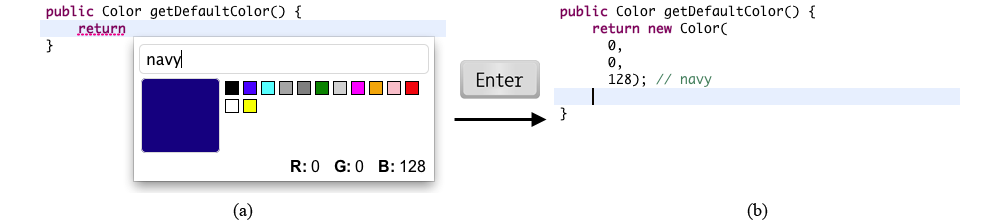
\includegraphics[width=35pc]{color_palette.png}\end{center}
\caption{This figure, reproduced from the prior work \cite{DBLP:conf/icse/OmarYLM12}, shows (a) a simple example GUI associated with the \texttt{Color} type, and (b) the code generated by this GUI once the ephemeral interaction is complete.}
\label{fig:color}
\end{figure*}

\begin{figure*}[t!]
\begin{center}
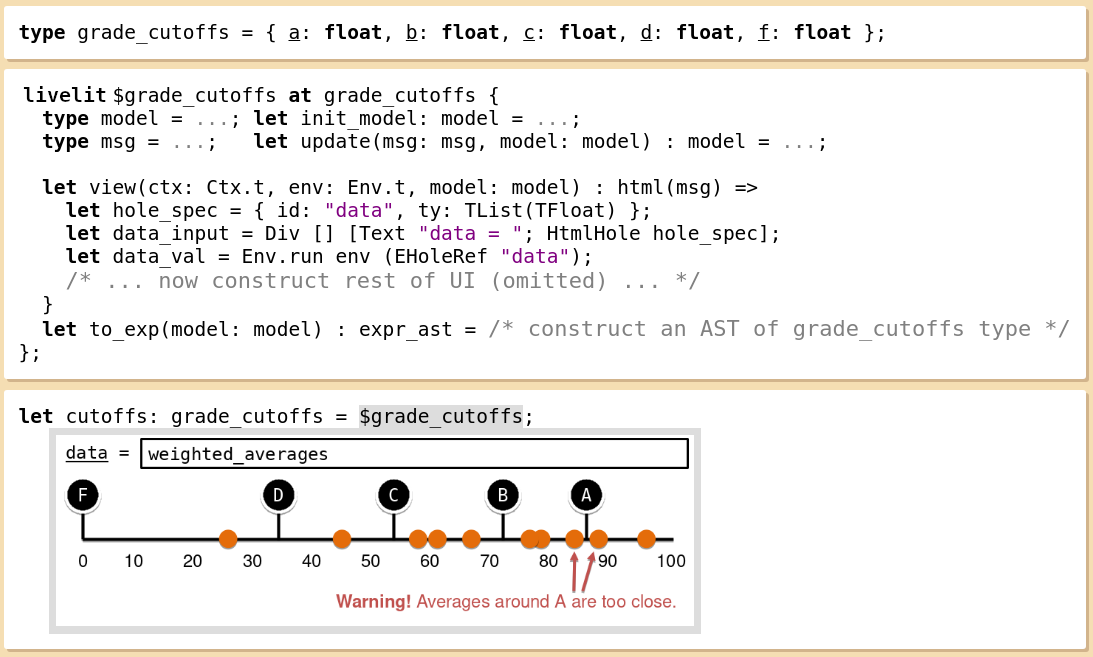
\includegraphics[width=34pc]{cutoffs-mockup.png}\end{center}
\caption{A mockup of a livelit for adjusting grade cutoffs. Livelits are persistent and can access the live environment.}
\label{fig:cutoffs}
\end{figure*}

There are two major limitations with this prior work. 
First, GUIs in Graphite are \textbf{ephemeral}, i.e. they disappear once the initial interaction is complete, leaving behind only the textual representation. This means that feedback and assistance is available only to the programmer
that first writes the code. 
% Graphite does include an \emph{ad hoc} mechanism that allows palettes to parse user-selected code when the GUI loads, but this requires significant additional effort. 

Second, Graphite does not provide any compositional way to {enter subexpressions within the GUI}.
This implies that Graphite's GUIs can only generate \textbf{closed expressions}. For example, in Figure~\ref{fig:color}, there is no way to specify that the \texttt{R}, \texttt{G}, or \texttt{B} values of the color being entered should be computed by a specified expression---only closed colors are supported. 
% This limitation precludes a variety of other perhaps more interesting use cases, e.g. GUIs for entering tabular data where each entry in
% the table is an arbitrary expression of the appropriate type. It also precludes nested composition of GUIs, e.g. a table where some entries are numbers generated by manipulating a slider GUI.

\vspace{-6px}
\section{Livelits}
\vspace{-2px}
To address these limitations, we introduce live literals, or livelits. Figure~\ref{fig:cutoffs} shows a mockup of the definition and application of a livelit named \li{$grade_cutoffs} for adjusting grade cutoffs, represented as values of  record type \li{grade_cutoffs}. Like textual literal forms (e.g. list literals), livelits are alternative representations of expressions of the associated type \cite{DBLP:journals/pacmpl/OmarA18}. % From the perspective of the remainder of the program, \li{cutoffs} is a value of type \li{grade_cutoffs} like any other.
We are implementing livelits in Hazel (\url{hazel.org}), a live functional programming environment with support for typed holes \cite{popl-paper}. We plan to perform a live demo.




The definition of
the livelit, outlined in Figure~\ref{fig:cutoffs}, follows the Elm architecture,
i.e. there are types representing the abstract model and the messages that the 
GUI generates. Livelits are \textbf{persistent} rather than ephemeral, i.e. the model is recorded in the underlying syntax tree. The \li{view} function generates the GUI, implemented using HTML, on demand (so the view is not persisted). Another function, \li{to_exp}, is responsible for generating the underlying expression, called the \emph{expansion}, from the \li{model}. 
While other projectional editors, e.g. those generated by Citrus \cite{DBLP:conf/uist/KoM05}, also support persistent GUIs in code, they are not user-extensible. 

The GUI can itself contain typed holes, represented by the \li{HtmlHole} constructor. In this case, there is a single hole
for entering an expression of type \li{list(float)}, i.e. the list of weighted
averages. In this example, the user has filled this hole with a variable,
\li{weighted_averages} (the definition of which is not shown). In other words,
livelits support \textbf{open expressions} and therefore interact cleanly with 
standard abstraction mechanisms, i.e. they can appear under binders. We follow the reasoning principles for literals with spliced sub-expressions established  by \citet{DBLP:journals/pacmpl/OmarA18}.

The main complication when dealing with open expressions relates to how live feedback
is to be generated. Given just the symbolic expression in the hole, it would be 
impossible to plot (as orange dots) the actual data from the list that the variable refers to. To resolve this issue, the system evaluates the program 
as if it the livelits were empty holes, 
relying on the support for evaluating incomplete programs described recently 
by \citet{DBLP:journals/pacmpl/OmarVCH19}. The result of evaluation is an expression containing
hole closures, i.e. holes equipped with environments. 
%Hazel allows the user to interactively select which closure
%interests them if multiple closures for a given hole appear in the result (e.g. if a livelit appears inside a function called multiple times). 
The livelit 
can then evaluate the expression in the hole against the closure selected by the user (not shown) using \li{Env.run}.


\clearpage
\bibliography{references,all.short,hazel_NSF}

% \clearpage
% \appendix
% \input{implementation-appendix}

\end{document}
